\documentclass[10pt,twocolumn,letterpaper]{article}
\usepackage[margin=0.7in,columnsep=0.25in]{geometry}
\usepackage{times}
\usepackage[T1]{fontenc}
\usepackage{graphicx,booktabs,amsmath,multirow,array,xcolor,enumitem}
\usepackage[hidelinks]{hyperref}
\usepackage{caption}
\usepackage{balance}
\captionsetup{font=small,labelfont=bf,skip=3pt}
\setlist{itemsep=0pt,topsep=1pt,parsep=0pt,leftmargin=11pt}
\usepackage{titlesec}
\titlespacing*{\section}{0pt}{5pt}{2pt}
\titlespacing*{\subsection}{0pt}{3pt}{1pt}
\titleformat*{\section}{\normalsize\bfseries}
\titleformat*{\subsection}{\small\bfseries}
\setlength{\textfloatsep}{6pt}
\setlength{\floatsep}{5pt}
\setlength{\dbltextfloatsep}{6pt}
\renewcommand{\arraystretch}{1.02}
\newcommand{\dec}[1]{\par\noindent\textit{Decision:} #1\par}

\title{\vspace{-1.6em}\large\textbf{Phase 1: FIFO Baseline for Memory-Aware Scheduling of Multi-Step Agents}\vspace{-1.8em}}
\author{}
\date{}

\begin{document}
\maketitle

\section{Project Description and Setup}
Our objective is to determine whether a scheduler that anticipates memory demand and agents returning from tool calls can beat FIFO on throughput and task latency under a fixed memory budget. In Phase~1, we implemented FIFO with fixed concurrency $N$, measured it across several configurations to select a baseline, and collected preliminary memory, runtime, tool-wait, and recomputation measurements to inform Phase~2.

\textbf{System.} The GPU platform used for baseline runs was NVIDIA T4 GPU on AWS EC2 instance.
We hosted a \texttt{llama-server} to serve Qwen3-0.6B Q8\_0 with \texttt{f16} KV in a \emph{unified} KV pool (\texttt{-kvu}, \texttt{-np}$=N$), where prompt caching was kept on while host cache was turned off. For our model, one token costs 112\,KiB of KV cache, so our \textit{fixed} 32K token KV pool reserves 3.5\,GiB at startup. These configurations were determined after running a series of smoke tests, as described later.

\textbf{Workload.} We replayed the AgentTrace tasks (MBPP, NL2Bash) using the scaled wait times ($150\times$, capped at 10\,s) for its tools, used greedy decoding and fixed output budgets as per the dataset. Time scaling was required to ensure the realistic tool call scenarios, as the dataset provide minimal wait times for tools in $ms$. We process the next scheduled request in the FIFO queue whenever a GPU worker becomes available, i.e., when fewer than $N$ concurrent requests are running on the GPU. A task frees its slot during tool waits but its KV cache may stay resident.

\textbf{Metrics.} We consider serveral metrics in this experiment. The most important once include the amount of tasks completed, throughput (completed tasks/min), \textit{successful} task p50/p95 end-to-end latency (s), queue wait (s), physical KV occupancy and cache reuse.

\section{Initial smoke tests and directions}
% \textbf{S1 -- Feasibility (10 burst runs).} We initially took L4 6GiB GPU. It completed only 2--10 of 50 tasks with a 16K tokens KV pool and 34/50 with 32K pool at $N{=}8$. Onsweep the T4 completed 550/550 task executions vs.\ 468/550 on the L4, with a 23\,s vs.\ 767\,s median at $N{=}2$. T4 device memory stayed flat at 4.4\,GiB because KV is preallocated.
% \dec{T4 with a 32K unified pool; any failure is then due to the KV budget, not device memory.}

\textbf{S1 -- L4 slice versus full T4 comparison.} In order to gauge the optimal experimental settings and configuration, we performed 11 smoke tests on L4 and T4 GPU. In initial L4 smoke runs, a 16K KV pool completed 10/50 tasks at \(N=8\) and 2/50 at \(N=16\). This indicated towards increasing the KV cache pool size to 32K, resulting in completion of 34/50 tasks at \(N=8\). We ran 11 configurations on each platform, replaying the same 50 tasks in every configuration. The L4 slice completed 468/550 task executions, compared with 550/550 on the full T4. At \(N=2\), median end-to-end task completion time was 767.4 seconds on the L4 and 23.3 seconds on the T4.
\dec{Use the T4 with a 32K unified KV pool for baseline runs.}

% \textbf{S2 -- Evaluating Concurrency Limits Under Realistic Request Arrivals (T4, Poisson 40\,s, $N{=}$1--16).} All levels completed 50/50 at near-identical throughput (1.52--1.56/min); at most five requests were ever active. Turning off prompt reuse raised prefill 9.4$\times$ but moved median latency by only 1.5\,s; removing tool delays moved it by 1.0\,s.
% \dec{Arrivals must be much faster to distinguish $N$. Generation dominates service time.}

\textbf{S2 -- Evaluating Concurrency Limits Under Realistic Request Arrivals (T4, Poisson 40\,s, $N{=}$1--16).} All configurations completed 50/50 tasks at nearly identical throughput (1.52--1.56 tasks/min), with at most five requests active simultaneously. This suggests that the 40-second arrival interval was too sparse to saturate the configured concurrency levels, making \(N\) largely irrelevant under this workload. Disabling prompt reuse and removing tool delays changed median task latency little under this light load, suggesting that generation dominates service time; the ablation results are detailed below.
\dec{Increase the arrival rate to create higher concurrency, saturate the GPU, and expose the impact of $N$ on throughput and latency.}

% \textbf{S3 -- Instrumented grid ($N\in\{2,4,8,16\}\times$ 3 arrival patterns, 50 tasks).} Table~\ref{tab:s3}. (i) For $N\ge4$ the pool hit 97--100\% occupancy while the GPU stayed at 4{,}383 of 15{,}360\,MiB; all 138 failures were KV-context errors. (ii) Completion depended on $N$, not arrivals, except at $N{=}16$. (iii) Burst $N{=}16$ had the highest throughput (4.80/min) by failing 32 of 50 tasks, so speed must be read with completion. (iv) Poisson runs never reached 16 active requests (max 11/14). (v) Only 32 size-only backfill opportunities appeared, none at $N{=}16$.

\textbf{S3 -- Narrowing search space grid ($N\in\{2,4,8,16\}\times$ 3 arrival patterns, 50 tasks).} We tested $(N=2,4,8,16)$ across three arrival patterns with 50 tasks per configuration (Table~\ref{tab:s3}, Figure~\ref{fig:s3-completion}). For $N\ge4$ the pool hit 97--100\% while GPU memory remained at 4{,}383 of 15{,}360\,MiB indicating that, as per our design, KV-context capacity in constrained memory bottleneck.  All 138 failures were KV-context errors. Task completion was largely determined by $N$, with little variation across arrival patterns except at $N=16$. Notably, burst traffic at $N=16$ achieved the highest throughput (4.80 tasks/min) but completed only 18/50 tasks, highlighting the trade-off between speed and reliability. With just 50 tasks, limited evidence on tail latency and failure rates, a $64K$ pool tested on only 20 tasks, and no zero-contention baseline, we need larger experiments to validate these trends.
\dec{Next, we scale to full tasks runs (500 tasks) with seven targeted configurations to better isolate concurrency, saturation, and scheduling effects.}

\begin{table}[h]
\centering\small
\caption{S3: tasks completed out of 50 (tasks/min), 32K pool.}
\label{tab:s3}
\setlength{\tabcolsep}{4pt}
\begin{tabular}{@{}lcccc@{}}
\toprule
Arrival & $N{=}2$ & $N{=}4$ & $N{=}8$ & $N{=}16$\\
\midrule
Burst & 50 (2.95) & 46 (3.38) & 34 (4.00) & 18 (4.80)\\
Poisson 5\,s & 50 (2.95) & 46 (3.26) & 34 (4.14) & 22 (4.11)\\
Poisson 10\,s & 50 (2.98) & 46 (3.41) & 34 (3.41) & 32 (3.55)\\
\bottomrule
\end{tabular}
\end{table}

\begin{table*}[t]
\centering\small
\setlength{\tabcolsep}{3pt}
\begin{tabular}{@{}cccc rrr rr r r r rr@{}}
\toprule
Run & $N$ & Arrival & KV & Done & Failed & Success & p50 (s) & p95 (s) & Tasks/min & Avg running & Avg KV & Peak KV & GPU MiB\\
\midrule
R1 & 1 & Pois.\ 10\,s & 32K & 500 & 0 & 100.0\% & 4{,}029 & 7{,}351 & 2.70 & 1.00 & 13.6\% & 49.0\% & 4{,}383\\
R2 & 4 & Pois.\ 5\,s & 32K & 480 & 20 & 96.0\% & 2{,}874 & 4{,}768 & 4.21 & 3.99 & 48.3\% & 99.9\% & 4{,}383\\
R3 & 16 & Pois.\ 5\,s & 32K & 177 & 323 & 35.4\% & 24 & 58 & 4.36 & 6.40 & 49.5\% & 100.0\% & 4{,}383\\
R4 & 4 & Pois.\ 2\,s & 32K & 472 & 28 & 94.4\% & 3{,}984 & 5{,}420 & 4.26 & 4.00 & 48.5\% & 99.9\% & 4{,}383\\
R5 & 16 & Pois.\ 2\,s & 32K & 100 & 400 & 20.0\% & 127 & 270 & 5.55 & 15.72 & 77.8\% & 99.9\% & 4{,}377\\
R6 & 4 & Burst & 32K & 476 & 24 & 95.2\% & 4{,}241 & 6{,}050 & 4.30 & 4.00 & 48.8\% & 99.9\% & 4{,}383\\
R7 & 16 & Pois.\ 2\,s & 64K & 340 & 160 & 68.0\% & 1{,}959 & 3{,}631 & 4.48 & 15.05 & 73.8\% & 100.0\% & 7{,}999\\
\bottomrule
\end{tabular}
\caption{Full-run results, 500 tasks. Latency is over successful tasks only. Avg and peak KV are the mean and maximum of one-second physical-occupancy samples, including retained idle contents, as percentages of the configured pool.}
\label{tab:full}
\end{table*}

\begin{figure}[t]
\centering
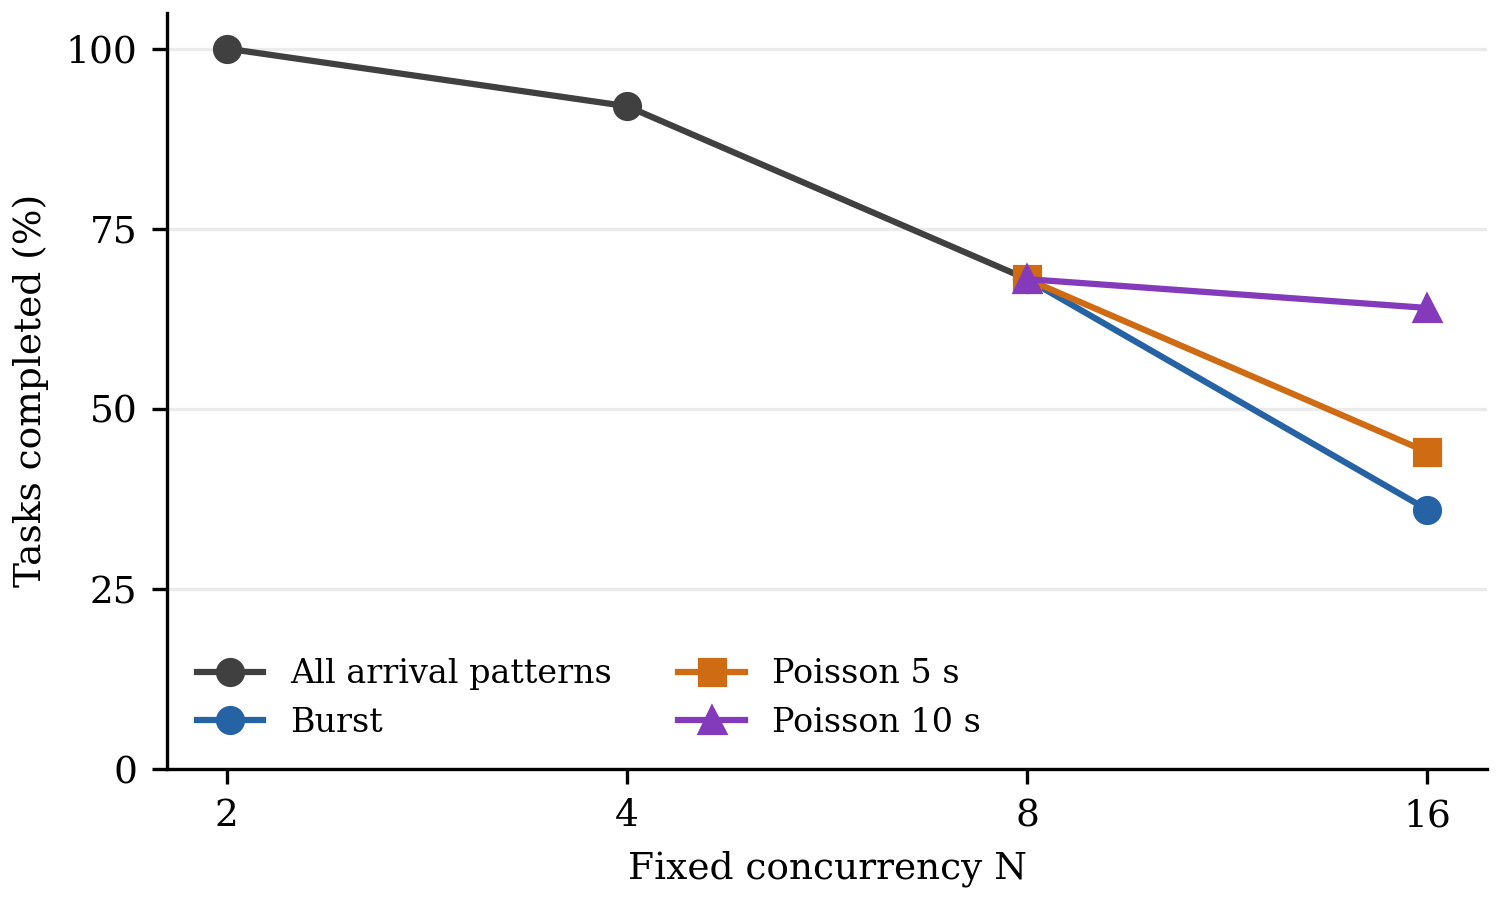
\includegraphics[width=\columnwidth]{fig_s3_completion.png}
\caption{S3 completion across concurrency levels for 50 tasks and a 32K KV pool. All three arrival patterns have the same completion rate at $N=2,4,8$.}
\label{fig:s3-completion}
\end{figure}

% \textbf{Gaps left open.} 50 tasks are too few for tail latency or failure rates (N2 vs.\ N4 differ by 4 tasks); $N{=}16$ was never saturated under Poisson; 64K was only tried with 20 tasks; there was no zero-contention reference.
% \dec{Scale to 500 tasks and run seven targeted configurations.}

\section{Full-Run Configurations}
The seven full runs replay the same 500-task trace (seed~2) with the same model, runtime, saved tool delays, and prompt-reuse setting. Based on the 50-task grid, we selected $N=1$ as a no-overlap reference, $N=4$ as the candidate FIFO baseline, and $N=16$ to stress KV capacity. We omitted $N=8$ to focus on these comparisons. The runs vary arrival pattern and include one 64K KV-pool configuration at $N=16$. We expected:
\begin{itemize}
    \item R1 to complete all tasks, while $N=4$ maintains high completion with a small, largely arrival-independent failure rate.
    \item $N=16$ to have substantially more failures, especially with faster arrivals.
    \item Increasing the KV pool to 64K to improve $N=16$ completion without necessarily eliminating failures.
    \item KV-context errors to remain the main failure cause, as they were in S3.
\end{itemize}

\section{Results}


\begin{figure}[t]
\centering
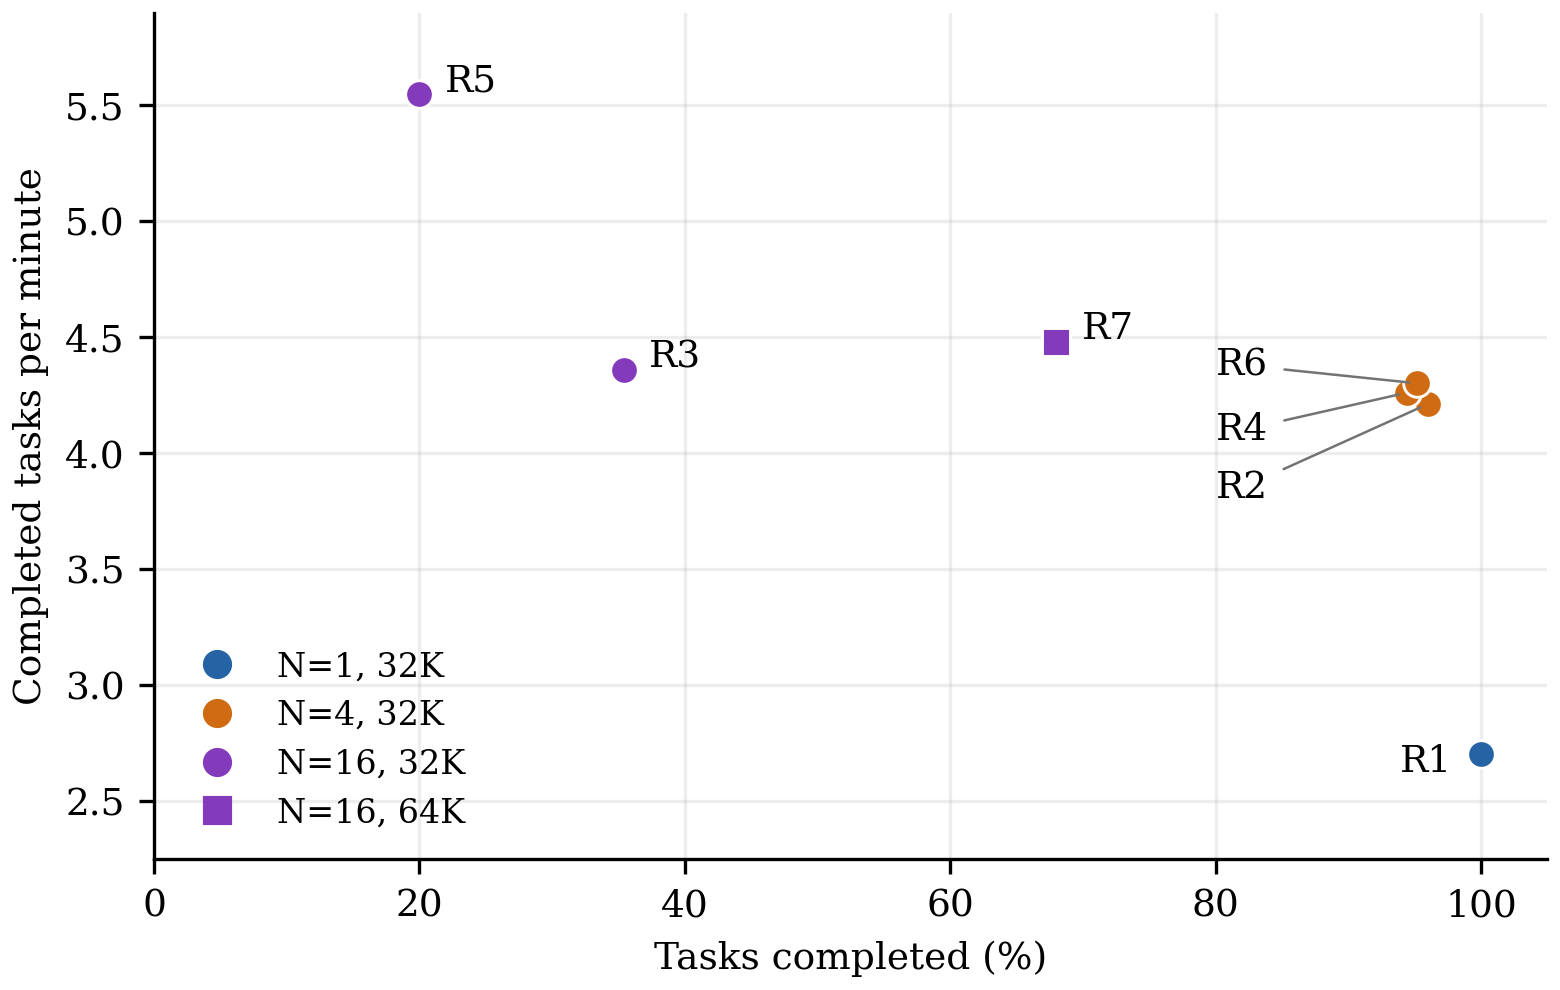
\includegraphics[width=\columnwidth]{fig_tradeoff_swapped.png}
\caption{Completion and throughput for the seven 500-task runs. Arrival patterns differ across runs; R7 uses a 64K KV pool.}
\label{fig:tradeoff}
\end{figure}

All the above expectations held (Table~\ref{tab:full}, Figure~\ref{fig:tradeoff}).
\begin{itemize}
\item \textbf{KV pool, not VRAM, is the bottleneck.} All 955 failures are KV-context errors, with no timeouts. Every $N\ge4$ run filled the pool while using at most 52\% of VRAM. Figure~\ref{fig:r4-kv} compares R4 and R5 occupancy over time.
\item \textbf{Context growth.} In the $N=4$ full runs, median prompt length grew from about 1.1K tokens on first requests to 3.1K on later requests. Later steps accounted for 70 of 72 KV-context failures. This associates growing contexts with pressure on the nearly full KV pool, although concurrency also affects whether a request fits.
\item \textbf{No task is infeasible in isolation.} R1 completed 500/500 with a 49\% peak KV utilization, confirming that failures arise from concurrent contexts competing for the KV pool.
\item \textbf{N4 remains stable across arrival patterns.} It achieved 94.4–96.0\% completion and 4.21--4.30 tasks/min under Poisson-5\,s, Poisson-2\,s and burst arrivals across two hosts, delivering 1.56–1.59$\times$ R1's throughput.
\item \textbf{N16 trades reliability for throughput.} Completion dropped to 35.4\% and 20.0\%, respectively. R5's 5.55 tasks/min came from just 100 successful tasks in an 18-minute run. Poisson-2,s reached 15.72 active requests, confirming that the stress test successfully saturated N16.
\item \textbf{More KV capacity improves completion but shifts the bottleneck.} Increasing the pool to 64K raised N16 completion to 68\%, but the larger pool also reached 100\% utilization, delivering only about 5\% more throughput than N4.
\item \textbf{Queueing dominates latency in the overloaded N4 runs.} Poisson-5\,s offered 12 tasks/min against 4.21 completed, and N4's ready-queue p95 reached 4{,}769--6{,}161\,s. This does not describe R3, whose ready queue was nearly empty.
\item \textbf{Prompt reuse.} In a separate, lightly loaded 50-task T4 comparison, disabling prompt reuse increased prefill tokens computed by 9.4$\times$, while median task latency rose from 32.8\,s to 34.3\,s. Both configurations completed all 50 tasks. Prefix reuse substantially reduced prefill work, although its effect on median end-to-end latency was small in this test.
\item \textbf{Tool waits and idle KV.} Tool waits in the 500-task trace had a median of 0.20\,s and a p95 of 4.46\,s. Removing delays in the light-load comparison reduced median task latency by 1.0\,s. In a separate T4 runtime validation, 127 KV cells remained occupied with no request processing and fell to zero after slot erasure. This confirms idle KV retention but does not quantify its effect on failures under load.
\end{itemize}

\balance
\section{Baselines and Phase~2 Plan}
\textbf{Baselines.} We selected N4 as the tuned FIFO baseline for its completion/throughput trade-off: 4.21--4.30 completed tasks/min with at least 94\% completion across the tested arrival patterns. N16 reached a higher measured tasks/min but failed many more tasks. N4's similar results across arrival patterns are preliminary because each full-run configuration was measured once. N1 serves as the zero-failure reference, completing all tasks without concurrent KV-context contention. Under the stricter objective of maximizing throughput while maintaining zero failures, only N1 currently qualifies. The Phase 2 target is to achieve a pareto-frontier on task completion-throughput compared to the N4 baseline, without skipping requests or shortening generated outputs.

% \textbf{Calibration status.}
% \emph{Request memory:} 112\,KiB/cell; prompt$+$max-output reservations disagreed with outcomes both ways in S3 (34 predicted fits failed, 127 predicted overflows succeeded), so a sharing/idle-cache correction and safety margin are needed.
% \emph{Run time:} outputs are fixed, so run time $\approx$ tokens$\times$TPOT$(N)$; burst TPOT was 9.9/16.0/24.4/31.2\,ms at $N{=}2/4/8/16$.
% \emph{Tool return:} median 0.12\,s, p95 3.7\,s per call, so the tool reserve should start small.
% \emph{Recompute:} 9.4$\times$ more prefill cost only 1.5\,s of median latency, so evicting idle caches is cheap. A slot erase returned occupancy to zero in validation; release under load is still untested.
% \emph{Backfill:} 23 opportunities in R2 and none at $N{=}16$; memory-aware admission should be tested first, with backfill as an increment.

\textbf{Phase 2 plan.} We will calibrate request-memory and runtime estimates, implement memory-aware admission, and test whether idle-cache eviction releases usable capacity under load. We will then test bounded-wait backfilling and compare the resulting scheduler with the N4 and N1 FIFO baselines across arrival rates and task mixes.


\clearpage
\onecolumn
\appendix
\section*{Additional Figures}
\noindent\begin{minipage}[t]{0.48\textwidth}
\centering
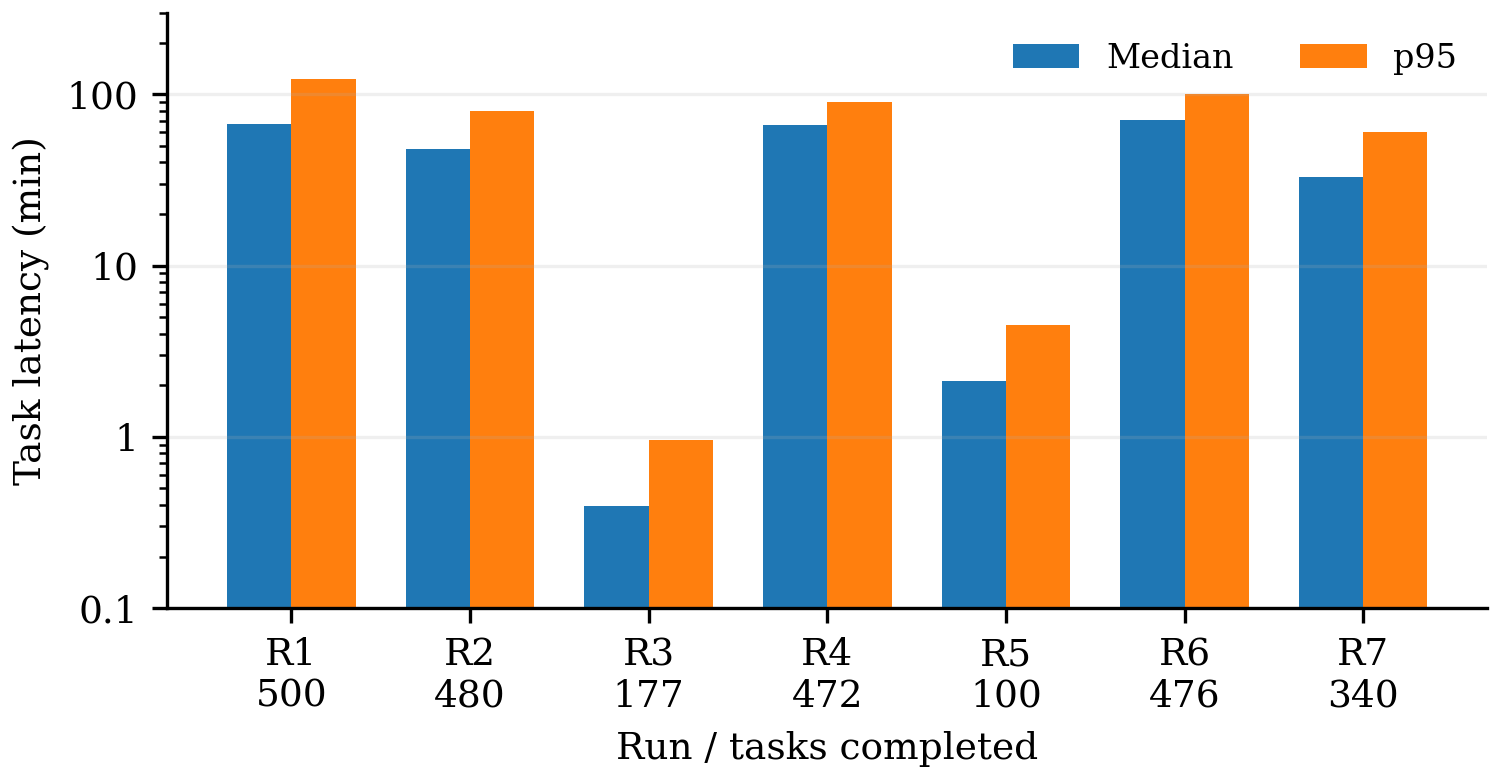
\includegraphics[width=\linewidth]{fig_latency_bars.png}
\captionsetup{font=scriptsize}
\captionof{figure}{Median and p95 latency for successful tasks across all seven runs. The vertical axis is logarithmic; counts below run labels are completed tasks out of 500.}
\label{fig:run-latency}
\end{minipage}\hfill
\begin{minipage}[t]{0.48\textwidth}
\centering
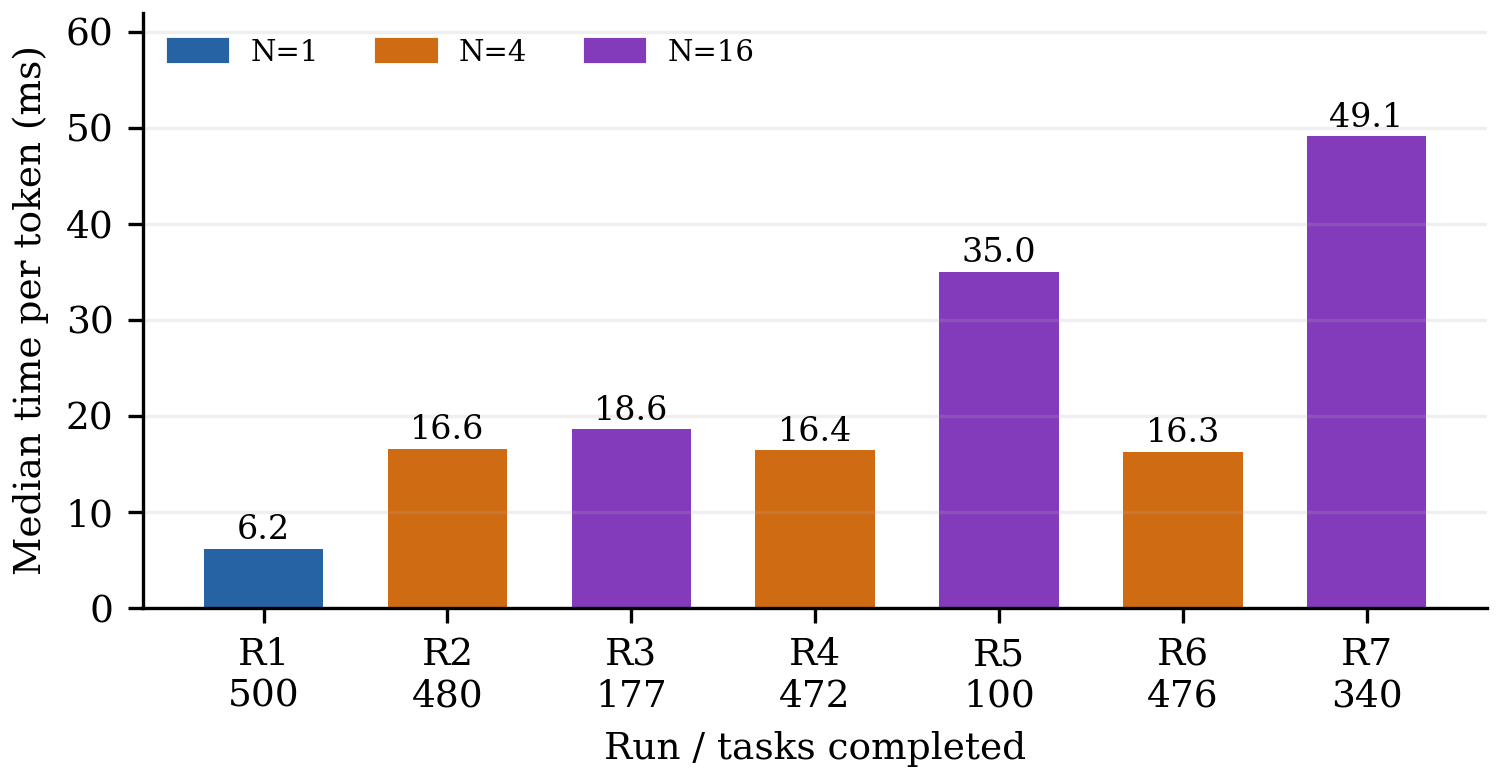
\includegraphics[width=\linewidth]{fig_full_generation_speed.png}
\captionsetup{font=scriptsize}
\captionof{figure}{Median time per output token across the seven full runs. Counts below run labels show completed tasks out of 500. Arrival patterns vary; R7 uses a 64K pool.}
\label{fig:generation-speed}
\end{minipage}

\begin{center}
\begin{minipage}{0.80\textwidth}
\centering
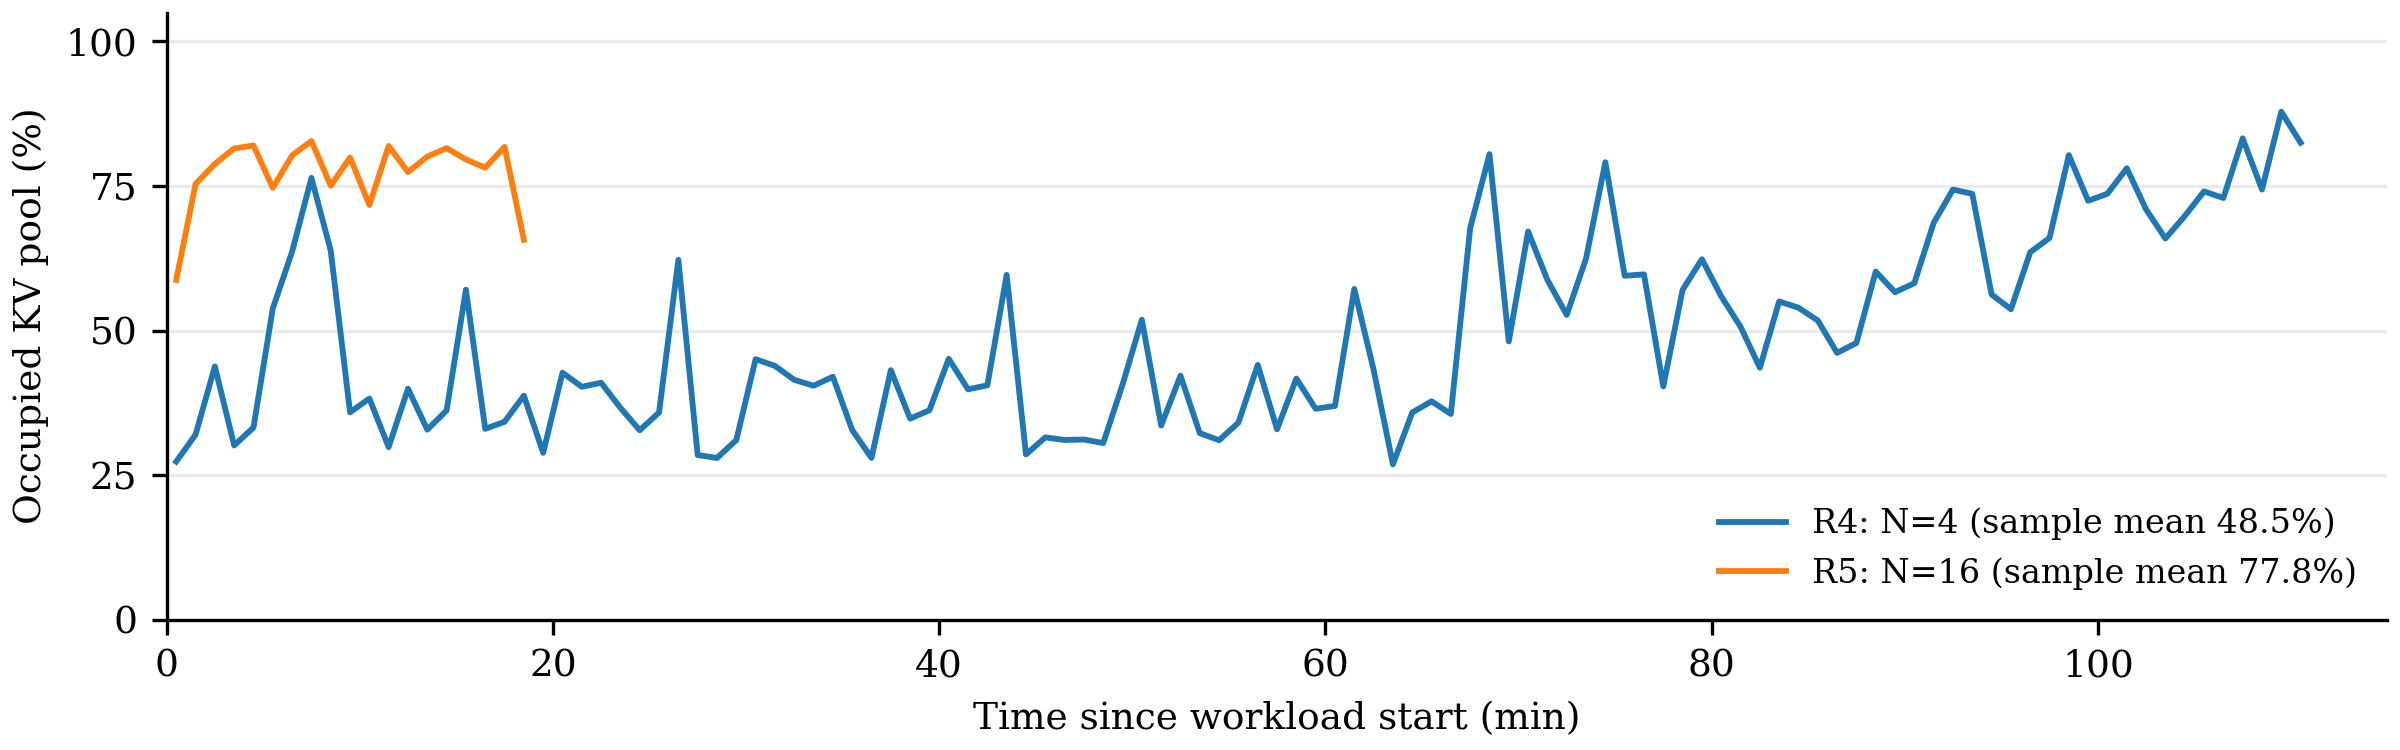
\includegraphics[width=\linewidth]{fig_kv_wide.png}
\captionsetup{font=scriptsize}
\captionof{figure}{R4 and R5 KV occupancy: one-minute means and overall sample means. Both use a 32K pool and Poisson 2\,s arrivals; R5 ends earlier. Occupancy includes retained idle contents.}
\label{fig:r4-kv}
\end{minipage}
\end{center}

\section*{Appendix A: Timeline and Milestones}
Completed dates are approximate. Final deliverable due \textbf{December 10, 2026}.

\begin{table}[h]
\centering\small
\renewcommand{\arraystretch}{1.25}
\begin{tabular}{@{}p{2.2cm}p{8.4cm}p{5.2cm}c@{}}
\toprule
Dates & Work & Milestone & Status\\
\midrule
\multicolumn{4}{@{}l}{\textbf{Phase 1: FIFO baseline and calibration}}\\
Oct 12--18 & Workload format and generator design; AgentTrace conversion & Replay workload format fixed & Done\\
Oct 19--25 & Phase~1 plan, FIFO replay harness, runtime benchmarks, and local smoke test & Harness runs end to end & Done\\
Oct 26--29 & AWS setup; L4 and T4 smoke tests and Poisson-40\,s sweeps & Platform chosen: T4, 32K unified KV & Done\\
Oct 29--31 & KV occupancy patch and validation; 12-run instrumented T4 grid & Binding resource identified (KV pool) & Done\\
Oct 31--Nov 1 & Seven 500-task full runs & FIFO baselines selected (N4, N1) & Done\\
Nov 2--4 & Phase~1 writeup and revision & Phase~1 report & Done\\
\midrule
\multicolumn{4}{@{}l}{\textbf{Phase 2: Predictive two-queue scheduler}}\\
Nov 9--15 & Exgentic adapter, dev/eval sets, and memory-aware FIFO admission & Memory-aware FIFO completes all dev tasks at N4-level load & Planned\\
Nov 16--22 & Backfill and aging; tool reserve, infeasible requests, and idle-cache eviction & Full scheduler runs on dev workloads & Planned\\
Nov 23--29 & Tune on dev runs, measure scheduler overhead, and freeze settings & Phase~2 settings frozen & Planned\\
\midrule
\multicolumn{4}{@{}l}{\textbf{Evaluation and final report}}\\
Nov 30--Dec 5 & Held-out comparisons with FIFO N4/N1 across arrivals and task mixes; repeat runs & Headline metrics: throughput, p95 latency, peak memory, failures, max queue wait & Planned\\
Dec 6--10 & Analyze estimation error, fairness, skipped tasks, and output length; prepare report & \textbf{Final report (Dec 10)} & Planned\\
\bottomrule
\end{tabular}
\end{table}

\end{document}
